%\section {Introduction}
%
%  Definition
%
\begin {frame} {Context}
  \centerline {
    \parbox {3cm} {
      Industrial robots
      \vskip .2cm
      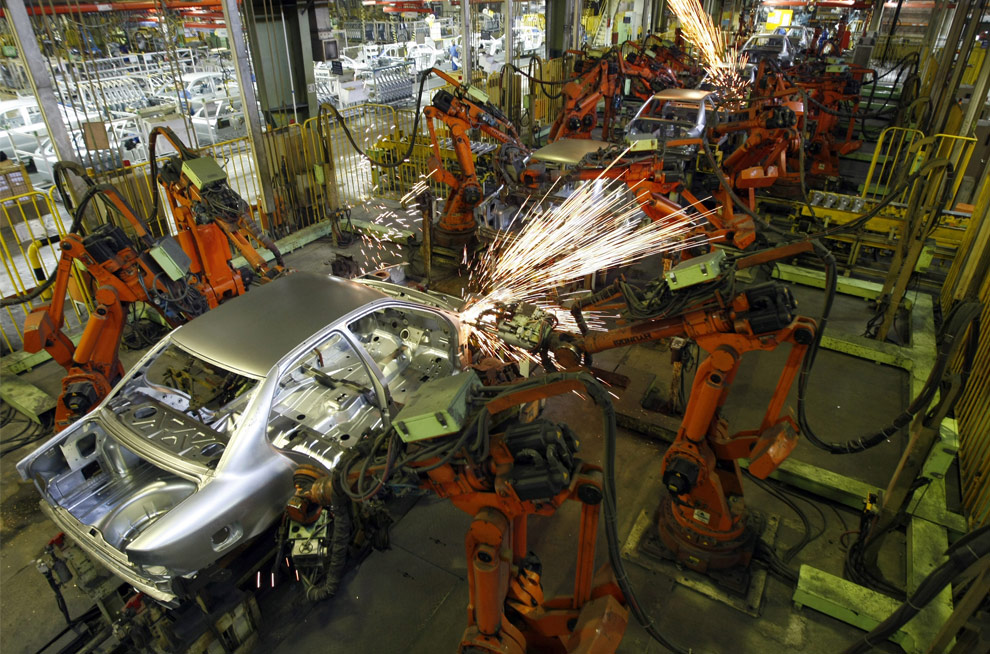
\includegraphics [height=2cm] {pictures/robot_welding_iran.jpg}
    }
    \hspace*{.05\linewidth}
    \parbox {3cm} {
      aerial robots
      \vskip .2cm
      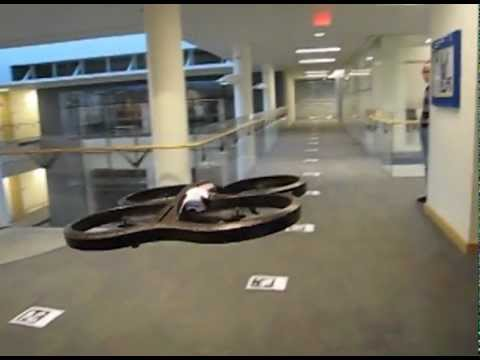
\includegraphics [height=2cm] {pictures/indoor-uav.jpg}
    }
    \hspace*{.05\linewidth}
    \parbox {3cm} {
      autonomous vehicles
      \vskip .2cm
      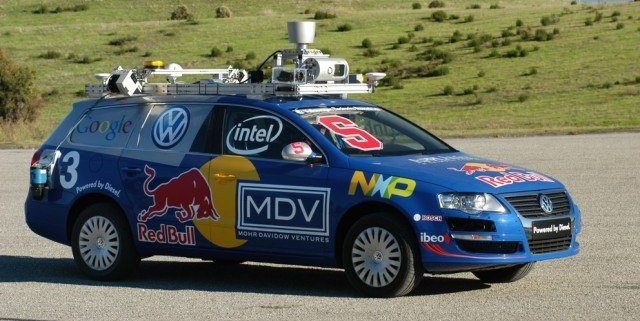
\includegraphics [height=2cm] {pictures/Google-robot-car.jpg}
    }
  }
  \vskip 1cm
  \pause
  Mobile autonomous system
  \begin{itemize}
    \item moving in an environment cluttered with obstacles
    \item subject to kinematic or dynamic constraints
  \end{itemize}
  \pause
  Motion planning~: automatically computing a feasible trajectory between two configurations.
\end {frame}
